\documentclass[12pt, a4paper]{article}

\usepackage{amsmath}
\usepackage[utf8]{inputenc}
\usepackage[spanish]{babel} %Paquete de idioma
\usepackage[hidelinks]{hyperref}
\usepackage{graphicx}
\usepackage{float}
\usepackage{eso-pic}
\usepackage{lipsum}
\usepackage{transparent}
\usepackage{parskip}
%\usepackage[backend=biber, style=apa]{biblatex}

\graphicspath{{images_doc/}}

%%%%%%%%% ESTO PARA LA MARCA DE AGUA %%%%%%%%%%%%%%%%%%%%%%%%%%%%%%%


\AddToShipoutPicture{ 
    \put(470,370){
        \parbox[b][\paperheight]{\paperwidth}{%
            \vfill
            \
            {
            \transparent{1}
            
\includegraphics[scale=0.1]{uware_logo.png}
            % 
\includegraphics[scale=0.5]{logo-ua.png}
            \vfill
            }
        }
    }
}
%%%%%%%%%%%%%%%%%%%%%%%%%%%%%%%%%%%%%%%%%%%%%%%%%%%%%%%%%%

\title{Detección de tuberías en imágenes submarinas} 


\author{
Leopoldo Cadavid Piñero
}








\begin{document}

\maketitle
\newpage
\tableofcontents
\newpage

      


\section{Preprocesamiento}\label{ch:preprocesamiento}

El preprocesamiento de la imagen constará de 2 partes:

\begin{itemize}
    
    \item Aplicar una mascara para aumentar el contraste. Esto se hace para compensar
    la distorsión en los colores provocada por la propagación de la luz a lo largo de la imagen.
    


    \item Posteriormente, se aplica un CAHE (o \textit{contrast-limited adaptive histogram equalization} ).
    con el objetivo de redistribuir la luminiscencia en la imagen. 
    
    

\end{itemize}

La aplicación de los métodos da como resultado una imagen mán nítida y contrastada
 donde es más fácil aplicar los algoritmos para la segmentación y detección de las estructuras.


\section{Deteccion de líneas}

\subsection{Primera aproximación}

Siguiendo con los métodos referenciados, se propone el uso de un filtro sobel para obtener
las respuestas de gradiente, y añadir esta respuesta de gradiente a un vector de características,
con el objetivo de dividir la imagen según estas características en diferentes clusters. Para ello se pretende usar el algoritmo
k-means. 

\textbf{Primeros resultados:} tras aplicar el método descrito, las clusterización no arroja una segmentación prometedora.
Los fallos posibles:
\begin{itemize}
    \item Que los bordes no sean una características significativa a la hora de detectar
    el objeto. 

    \item Una implementación errónea del algoritmo a partir de la descripción. 
    \item Una representación errónea de los datos.
\end{itemize}


-Tras la comprobación de las distintas transformaciones aplicadas a la imagen, se observa que la conversión de escala rgb a escala 
de grises provoca una gran perdida de información, afectando esto al uso del algoritmo Sobel, pues se pierde información importante del cambio de 
gradiente en ciertos canales de color de la imagen.

A raíz de esto, se ha aplicado el filtro sobel a cada uno de los canales de la imagen por separado. Posteriormente, se calcula el gradiente medio de cada
canal y se añade cada uno al algoritmo k-means. De esta forma se ha conseguido mejorar sustancialmente la clusterización. Aún así, no es suficiente como para que 
haya separado la tuberia en la imagen de referencia. 

Lo proximo a tratar será la detección de lineas en cada una de las imagenes de gradiente, para ver si estas facilitan el proceso de segmentado.

\subsection{Segunda aproximación}

En este caso, tomando como base ciertas ideas comentadas en la anterior aproximación, 
se trata de conseguir la detección de forma distinta al paper estudiado. Los pasos seguidos 
en este caso han sido los siguientes: 

\begin{itemize}
    
    \item Realizar el preprocesamiento, tal y como se describe en \Ref{ch:preprocesamiento}.
    
    \item Aplicar un filtro bilateral para eliminar cierto ruido del fondo de las imágenes.
    
    \item Aplicar el algoritmo \verb|PyrMeanShift()|, para que la imagen quede segmentada por colores.
    
    \item Aplicar el  algoritmo \textbf{Sobel()}, a cada uno de los canales de la imagen 
    RGB preprocesada. Esto se hace para obtener los cambios de gradiente y se aplica por igual 
    a los ejes X e Y, realizando una suma ponderada de ambos con el fin de obtener el 
    cambio en distintas direcciones. 

    \item Obtener, a partir de los gradientes, bordes en las imágenes aplicando el 
    algoritmo \verb|Canny()|.

    \item Utilizamos filtros morfológicos para erosionar y dilatar, tratando de eliminar,
    elementos circulares que puedan molestar y amplificando los elementos rectangulares.

    \item Teniendo los bordes filtrados, se utiliza la transformada de Hough para encontrar líneas en 
    dentro de la imágen.

    \item A partir de los 3 vectores de líneas que tenemos, creamos uno nuevo donde juntaremos
    \textbf{todas la líneas de la imagen}. 
    
\end{itemize}

\begin{figure}[H]
    \centering
    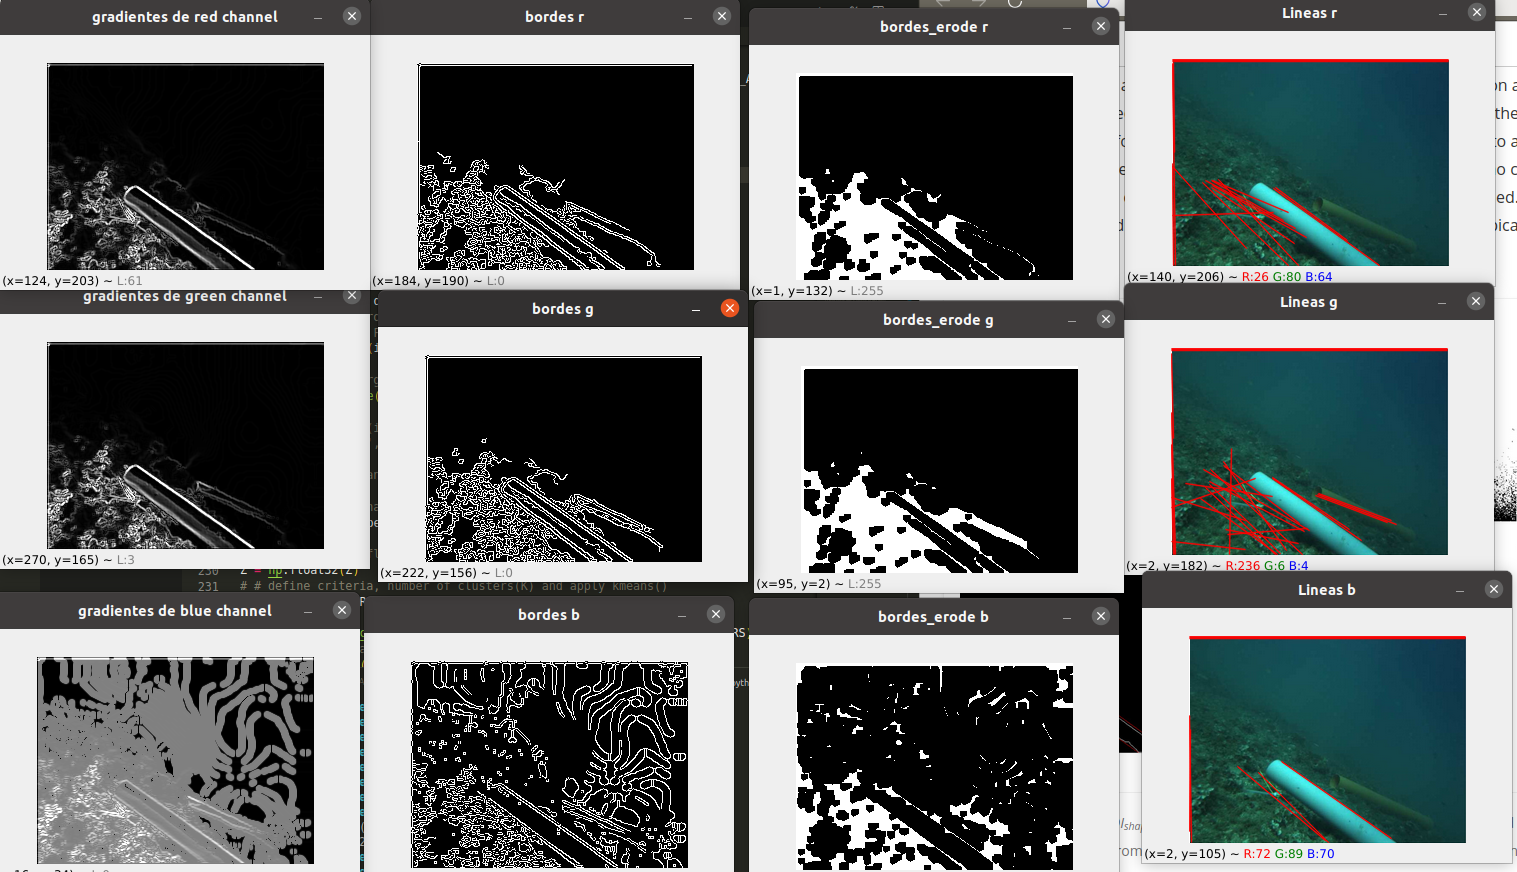
\includegraphics[scale=0.3]{sobel_canny_houghlines.png}
    \caption{Líneas obtenidas para cada canal en una de las imágenes estudiadas}
    \label{fig:sobelcanny}
\end{figure}

\section{Filtrado de líneas}



\section{Referencias}

https://journals.sagepub.com/doi/10.5772/60526

% \begin{figure}[H]
%     \centering
%     \includegraphics[scale=0.1]{tarea_1roscore.png}
%     \caption{Lanzamos el master}
%     \label{fig:tarea1roscore}
% \end{figure}



\end{document}